\documentclass[conference]{IEEEtran}
\usepackage{cite}
\usepackage{amsmath,amssymb}
\usepackage{graphicx}
\usepackage{booktabs,array}
\usepackage{algorithmic}
\usepackage{tikz}
\usetikzlibrary{arrows.meta,positioning,shapes.geometric}
\usepackage[hidelinks]{hyperref}
\urlstyle{same}
\newcounter{paperalgorithm}
\newcommand{\sys}{TrailGuard TW}
\newcommand{\tool}[1]{\texttt{#1}}
\begin{document}
\title{TrailGuard TW: An Evidence-Grounded MCP Architecture for Mountain Trip Planning in Taiwan}
% Replace the author block before submission. Do not infer author identities.
\author{\IEEEauthorblockN{Author Name(s)}
\IEEEauthorblockA{Department and Institution\\City, Taiwan\\Corresponding author email}}
\maketitle
\begin{abstract}
Mountain trip planning combines route characteristics, forecasts, access restrictions, and team capabilities whose spatial and temporal scopes may not agree. A fluent recommendation can therefore be unsupported even when it cites relevant documents. This paper proposes TrailGuard TW, an evidence-grounded decision-support architecture for mountain trips in Taiwan. A language model elicits requirements and coordinates typed Model Context Protocol (MCP) tools, while deterministic functions compute derived values and enforce restrictions. Temporal evidence records link observations to route segments, effective intervals, and computation histories. Before candidate ranking, a three-state gate distinguishes prohibited itineraries (NO-GO), unresolved essential evidence (HOLD), and candidates passing the configured checks (ADMISSIBLE). The design specifies eight modules, tool contracts, a bounded planning algorithm, and an auditable output package. A structured comparison relates the architecture to retrieval-augmented generation and tool-using agents. A planned evaluation combines 90 route--team scenarios and 30 adversarial cases, with controlled baselines and explicit metric denominators. Synthetic traces illustrate intended behavior; they are not experimental results. This work contributes a reproducible system specification and evaluation protocol, while leaving implementation, field validation, and measured effectiveness to future study.
\end{abstract}
\begin{IEEEkeywords}
large language models, Model Context Protocol, retrieval-augmented generation, decision support, temporal evidence, mountain trip planning
\end{IEEEkeywords}

\section{Introduction}
Planning a mountain trip involves decisions whose supporting information changes at different rates. Route geometry may remain stable while trail access, forecasts, water availability, and team readiness change rapidly. A useful planning assistant must connect these observations to the proposed travel dates and route segments, explain missing information, and distinguish an admissible plan from an unsupported recommendation. Taiwan provides the geographical setting for the proposed system, rather than a basis for assuming uniform conditions across all mountain routes.

The motivating problems are fragmented information and difficulty judging retreat conditions. We propose a domain agent combining a large language model (LLM), Python analytics, temporal knowledge, and an evidence ledger. An explicit MCP boundary separates the planner from its tools. This paper specifies the architecture and its evaluation protocol; it does not report a deployed implementation or measured performance.

Retrieval-augmented generation (RAG) supplies external documents to a generator~\cite{rag}, while reasoning-and-acting approaches combine language-model planning with external interactions~\cite{react}. These capabilities motivate a conversational interface, but neither citation establishes that retrieved passages are current or that a generated itinerary obeys domain constraints. A planning system therefore needs explicit data validation and a decision layer whose result cannot be overridden by fluent generated text.

This paper asks: \emph{How can a mountain-planning assistant expose heterogeneous tools to an LLM while preserving temporal relevance, numerical provenance, and non-negotiable restrictions?} We propose three design contributions: (1) an eight-module architecture with MCP tool contracts and a bounded orchestration process; (2) a temporal evidence ledger coupled to a three-state decision gate; and (3) an evaluation protocol that measures unsafe approvals, unsupported claims, and service failures separately from usability. These are proposed mechanisms and testable hypotheses, not demonstrated improvements over existing systems.

The work fits research on applied AI, knowledge engineering, information retrieval, and intelligent planning. Its immediate deliverable is an inspectable design. Demonstrating operational utility requires implementing adapters, curating reference cases, and conducting the experiments described below.

\section{Related Work and Design Rationale}
\subsection{Retrieval and Tool-Using Agents}
RAG combines a language model with external retrieval~\cite{rag}. In this design, retrieval supports domain explanations and document-level evidence. Structured feeds remain the preferred input for machine-readable restrictions and numeric observations when available. A retrieved passage is not automatically accepted as an authoritative operational record.

ReAct studies interleaving reasoning and actions to obtain information from external environments~\cite{react}. TrailGuard TW adopts task decomposition and tool interaction as design principles. However, it places admission decisions in explicit rules rather than allowing the LLM to infer unrestricted exceptions. The proposed separation makes errors in slot extraction, data acquisition, numerical analysis, and explanation independently observable.

MCP defines interfaces through which servers expose named tools, input schemas, and tool results~\cite{mcp}. It is a tool-interoperability mechanism; it does not certify source correctness or enforce the application-specific decision policy. Our proposed use of MCP is to standardize the boundary between the LLM host and data or computation services. Direct API access could implement similar domain logic; whether MCP improves adapter maintainability is an empirical engineering question.

\subsection{Comparison of Agent Design Patterns}
ReWOO separates planning from observations to reduce repeated reasoning over tool outputs~\cite{rewoo}. Reflexion uses verbal feedback and episodic memory to improve subsequent attempts~\cite{reflexion}. LLMCompiler organizes function calls into an execution plan that can exploit parallelism~\cite{llmcompiler}. These approaches offer useful orchestration patterns, but their reported benchmark results do not establish compliance with mountain-specific restrictions.

Table~\ref{tab:related} compares the mechanism of each reference with the additional checks required by this application. Its final column is our design analysis, not a claim that the cited work fails its own objectives. TrailGuard TW combines existing patterns with a domain-specific gate and provenance contract; novelty and effectiveness of the combination remain to be evaluated. Independent weather and access queries could be scheduled concurrently, but every response must pass the same temporal and schema checks before use.

\begin{table*}[t]
\caption{Related Mechanisms and Their Role in the Proposed Design}
\label{tab:related}
\centering\footnotesize
\begin{tabular}{@{}p{0.15\textwidth}p{0.24\textwidth}p{0.25\textwidth}p{0.28\textwidth}@{}}
\toprule
Reference / approach & Main mechanism & Role in TrailGuard TW & Additional application requirement\\
\midrule
RAG~\cite{rag} & Generate with retrieved external evidence. & Retrieve guidance and explanatory passages. & Check source authority, route scope, and effective time.\\
ReAct~\cite{react} & Interleave reasoning with external actions. & Clarify inputs and select data tools. & Bound tool calls and separate admission from explanation.\\
ReWOO~\cite{rewoo} & Decouple planning from observations. & Inform reusable acquisition plans. & Replan when essential evidence is missing or conflicting.\\
Reflexion~\cite{reflexion} & Use verbal feedback in episodic memory. & Inform offline error analysis and prompt revision. & Feedback must not rewrite authoritative restrictions.\\
LLMCompiler~\cite{llmcompiler} & Schedule dependent and parallel function calls. & Inform concurrent independent acquisition. & Validate all results before the decision gate.\\
MCP~\cite{mcp} & Discover and invoke schema-defined tools. & Standardize adapter interfaces. & Enforce domain semantics in the application.\\
TrailGuard TW (proposed) & Temporal evidence, deterministic gate, and ledger. & Integrate the above roles for mountain planning. & Requires implementation and independent empirical evaluation.\\
\bottomrule
\end{tabular}
\end{table*}

\subsection{Domain Evidence and Temporal Relevance}
The Central Weather Administration (CWA) publishes an open-data API guide~\cite{cwa}. This establishes a candidate acquisition channel, not an implemented TrailGuard TW integration or a guarantee that every route has suitable forecast coverage. Each deployed adapter must document the selected dataset, credentials, spatial resolution, update behavior, and permitted use. Trail restrictions and water reports similarly require individually verified providers; this paper does not claim a universal trail-status API.

The architecture treats weather, access restrictions, route records, water reports, and approved domain guidance as distinct evidence classes. A general document about mountain illness must not be converted into an individual diagnosis or an unvalidated numerical risk score. A disclosed medical history may trigger additional questions or referral under an expert-approved rule set. Such rules remain a deployment dependency.

Three tensions guide the design: flexibility versus rule enforcement, experiential estimates versus reproducible calculation, and candidate diversity versus conservative handling of uncertainty. We resolve these tensions procedurally: collect preferences conversationally, compute with versioned functions, apply restrictions before ranking, and preserve uncertainty in the output. The architecture is intended to support decisions, and its admissibility label is not a guarantee of real-world safety.

\section{Problem Formulation and Requirements}
\subsection{Inputs, Candidates, and Decision States}
A request is represented as
\begin{equation}
 x=(r,[t_0,t_1],n,e,p,m),
\end{equation}
where $r$ is the requested route, $[t_0,t_1]$ the travel interval, $n$ the team size, $e$ experience descriptors, $p$ stated preferences and pace information, and $m$ voluntarily supplied health-related flags. Missing essential fields cause a clarification request. Sensitive information is minimized in retained logs and is not sent to unrelated data tools.

A candidate itinerary $c$ is a sequence of route segments, arrival intervals, rest or overnight stops, and retreat checkpoints. Its evidence set is $E_c$. The decision state is one of $\{\text{NO-GO},\text{HOLD},\text{ADMISSIBLE}\}$. NO-GO means an applicable, verified rule prohibits the candidate. HOLD means essential evidence or required input is missing, stale, contradictory, or otherwise unresolved. ADMISSIBLE means the candidate passes the implemented checks with the available evidence; it does not assert comprehensive safety.

\subsection{Functional and Evidence Requirements}
Table~\ref{tab:modules} defines the eight functional modules of the proposed system. Five requirements connect them. First, missing dates or route identifiers must not be silently invented. Second, time-sensitive claims must carry validity intervals. Third, numerical outputs must be attributable to either a source observation or a documented computation. Fourth, prohibited candidates cannot be restored through weighted scoring. Fifth, failure to obtain essential evidence must be visible to the user.

\begin{table}[t]
\caption{Proposed Functional Modules}
\label{tab:modules}
\centering\footnotesize
\begin{tabular}{@{}p{0.29\columnwidth}p{0.65\columnwidth}@{}}
\toprule
Module & Responsibility and inspectable output\\
\midrule
User scenario & Define the planning question, intended users, and route context.\\
Query/input & Elicit dates, team size, experience, preferences, and required clarifications.\\
Planner/agent & Select bounded tool calls and track incomplete tasks.\\
Data acquisition & Retrieve provider records with temporal and spatial metadata.\\
Analytics engine & Compute segment times and evaluate versioned constraints.\\
Domain knowledge & Retrieve guidance and maintain temporal evidence relationships.\\
Decision / recommendation & Enforce NO-GO/HOLD gates before candidate ranking.\\
Output/interaction & Produce alternatives, checkpoints, and an evidence ledger.\\
\bottomrule
\end{tabular}
\end{table}

\section{Proposed Architecture}
\subsection{Layered Workflow}
Figure~\ref{fig:architecture} depicts the proposed execution boundary. The conversational planner first normalizes the request and checks required fields. The MCP host discovers approved tools and invokes them with validated arguments. Adapters return typed records; the evidence store validates their scope and provenance. The analytics engine computes derived values, and the rule gate assigns the decision state. Only admissible candidates proceed to ranking and explanation.

\begin{figure}[t]
\centering
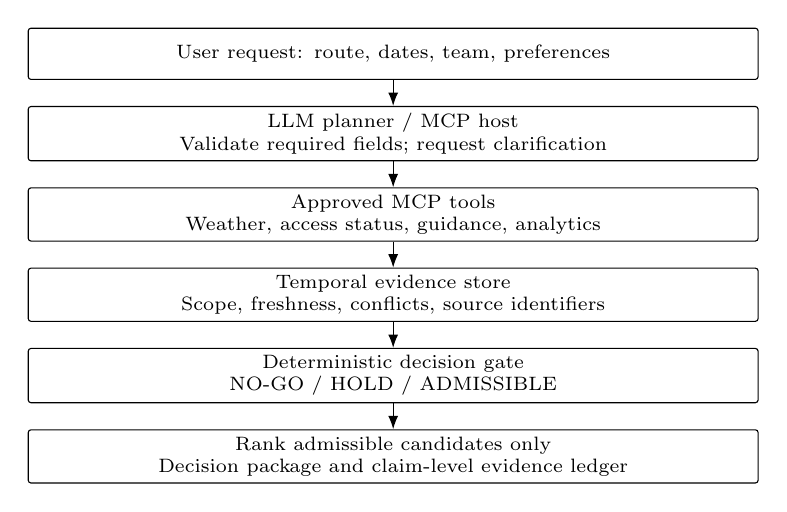
\begin{tikzpicture}[
 node distance=3.3mm,
 box/.style={draw,rounded corners=1pt,align=center,font=\scriptsize,
 text width=0.75\columnwidth,minimum height=6.5mm,inner sep=2.5pt},
 link/.style={-{Latex[length=1.7mm]},line width=0.45pt}]
\node[box] (input) {User request: route, dates, team, preferences};
\node[box,below=of input] (planner) {LLM planner / MCP host\\Validate required fields; request clarification};
\node[box,below=of planner] (tools) {Approved MCP tools\\Weather, access status, guidance, analytics};
\node[box,below=of tools] (evidence) {Temporal evidence store\\Scope, freshness, conflicts, source identifiers};
\node[box,below=of evidence] (gate) {Deterministic decision gate\\NO-GO / HOLD / ADMISSIBLE};
\node[box,below=of gate] (output) {Rank admissible candidates only\\Decision package and claim-level evidence ledger};
\draw[link] (input)--(planner);
\draw[link] (planner)--(tools);
\draw[link] (tools)--(evidence);
\draw[link] (evidence)--(gate);
\draw[link] (gate)--(output);
\end{tikzpicture}
\caption{Proposed flowchart. Rejected or unresolved candidates are explained but never enter the ranked recommendation set.}
\label{fig:architecture}
\end{figure}

The state sequence is \emph{input validation}, \emph{acquisition}, \emph{evidence validation}, \emph{analysis}, \emph{gating}, and \emph{presentation}. A failed step yields a typed error or a request for clarification. The orchestrator has a configurable tool-call budget, per-tool timeouts, and bounded retries. Exhausting the budget does not authorize filling evidence gaps with generated values.

\subsection{MCP Tool Contracts}
Table~\ref{tab:tools} lists proposed application tool names. They are design identifiers, not existing public services. After normal MCP initialization, the host can discover tool schemas and issue calls. Output validation must distinguish protocol failures, tool execution failures, empty results, and valid observations~\cite{mcp}.

\begin{table}[t]
\caption{Proposed MCP Application Interfaces}
\label{tab:tools}
\centering\footnotesize
\begin{tabular}{@{}p{0.43\columnwidth}p{0.51\columnwidth}@{}}
\toprule
Tool & Principal contract\\
\midrule
\tool{get\_weather} & Route geometry and interval to forecast records and coverage metadata.\\
\tool{get\_trail\_status} & Route identifier and interval to restrictions, notices, and effective dates.\\
\tool{get\_water\_reports} & Location and interval to dated reports with confidence descriptors.\\
\tool{retrieve\_guidance} & Query and scope filters to passages with document identifiers.\\
\tool{estimate\_segment\_time} & Validated segment and team inputs to estimates and computation lineage.\\
\tool{evaluate\_constraints} & Candidate, evidence IDs, and policy version to state and reason codes.\\
\bottomrule
\end{tabular}
\end{table}

For example, \tool{get\_trail\_status} accepts an object containing \tool{route\_id}, \tool{start\_time}, and \tool{end\_time}. Its structured result includes a status from \{open, restricted, closed, unknown\}, source URL, issued time, retrieved time, effective interval, and coverage description. A successful request that returns unknown is not equivalent to an open trail. The weather adapter must return units, forecast issue time, and applicable locations; the analytics adapter must reject incompatible units.

The host allowlists servers and tool names, validates arguments against schemas, and restricts calls to the resources needed for the task. Provider documents and retrieved passages are processed as data, not as instructions that can change tool permissions or decision rules. Credentials stay in adapter configuration rather than prompts or exported ledgers. These are proposed application controls, not properties supplied automatically by MCP.

\subsection{Temporal Evidence Representation}
Each evidence item is represented as
\begin{equation}
 e_i=(\iota_i,s_i,u_i,v_i,[a_i,b_i],q_i,h_i),
\end{equation}
where $\iota_i$ is an identifier, $s_i$ the source, $u_i$ the retrieval time, $v_i$ the issue time, $[a_i,b_i]$ the effective interval, $q_i$ the spatial or route scope, and $h_i$ a content hash or snapshot identifier. Unknown endpoints must remain explicitly unknown. Acquisition time alone does not establish temporal applicability.

An item is eligible for a segment only when its scope matches that segment and its effective interval covers the relevant traversal time under the configured policy. A separate freshness check compares issue time with a provider-specific threshold. Thresholds are configuration values requiring provider and domain review; this paper does not prescribe a universal forecast age. Contradictory records are retained with their provenance. A conflict-resolution policy considers authority, effective time, and coverage, while unresolved essential conflicts produce HOLD.

A temporal knowledge graph links routes, segments, notices, forecast cells, and guidance documents through dated relations. Hybrid retrieval is proposed to combine lexical matching, semantic retrieval, and structured filters. Graph construction, embedding selection, and retrieval weights have not been implemented or benchmarked. The evidence ledger records which items support each output claim and how source values were transformed.

\subsection{Deterministic Analytics and Decision Gates}
For segment $j$, the engine computes a duration estimate
\begin{equation}
 \hat{\tau}_j=f_{\theta}(d_j,\Delta z_j,g_j,p),
\end{equation}
where $d_j$ is distance, $\Delta z_j$ elevation information, $g_j$ route attributes, and $p$ team pace information. The function and parameters $\theta$ must be documented and calibrated against independent observations. This specification does not select an established walking-time formula or claim validated coefficients. Reported intervals must identify their calibration basis; absent calibration, they remain engineering estimates.

Let $h_c=H(c,E_c)$ indicate an applicable authoritative prohibition, $u_c=U(c,E_c)$ unresolved essential information, and $k_c=C(c,E_c)$ satisfaction of all other required deterministic checks. The gate is
\begin{equation}
 D(c,E_c)=\begin{cases}
 \text{NO-GO},& h_c,\\
 \text{HOLD},& \neg h_c\land u_c,\\
 \text{ADMISSIBLE},&\neg h_c\land\neg u_c\land k_c,\\
 \text{NO-GO},&\text{otherwise}.
 \end{cases}
\end{equation}
An applicable closure is a direct example of $H$. Weather-related exclusions require a documented mapping from the authoritative warning's location and effective period to the candidate; a warning elsewhere must not automatically reject every route. Each rejection records the failed rule and its supporting evidence.

Ranking is performed only over $\mathcal F=\{c:D(c,E_c)=\text{ADMISSIBLE}\}$. Preference scores cannot offset a prohibition. When possible, the system returns up to three alternatives, described as conservative, balanced, and preference-oriented. All three alternatives remain subject to the same mandatory constraints. If fewer than three candidates are admissible, the system returns fewer; if none are admissible, it explains the blocking conditions.

A retreat checkpoint combines the estimated return duration, a documented time boundary such as a relevant daylight constraint, and an explicitly configured margin. Unsupported precision is avoided. Illness-related inputs trigger only reviewed guidance or referral logic; they are not converted by the LLM into medical clearance.

\subsection{Algorithm and Key Property}
Algorithm~\ref{alg:gate} gives the proposed control logic. A tool call consumes budget even if it fails; acquisition records errors rather than silently substituting observations. Candidate templates may be formed from cached route geometry, but admission still requires applicable evidence for the requested interval. No execution of this algorithm is claimed in the present study.

\begin{figure}[t]
\centering
\begin{minipage}{0.97\columnwidth}
\hrule\vspace{3pt}
\refstepcounter{paperalgorithm}\label{alg:gate}
\textbf{Algorithm \thepaperalgorithm: Bounded evidence-grounded planning}\par
\begin{algorithmic}[1]
\REQUIRE Request $x$, tool budget $B$, policy version $v$
\ENSURE Decision states, admissible set, evidence ledger
\STATE Normalize $x$ and check required fields
\IF{essential fields are missing}
\STATE \textbf{return} HOLD and clarification questions
\ENDIF
\STATE $E\leftarrow$ acquire approved evidence within budget $B$
\STATE Validate schemas, units, scope, freshness, conflicts
\STATE $\mathcal C\leftarrow$ generate candidate templates for $x$
\STATE $\mathcal F\leftarrow\emptyset$; initialize ledger $L$
\FOR{each candidate $c\in\mathcal C$}
\STATE Link relevant evidence $E_c$ and policy $v$ to $L$
\IF{an authoritative prohibition applies}
\STATE Record NO-GO and its supporting evidence
\ELSIF{essential evidence is unresolved}
\STATE Record HOLD and unresolved reason codes
\ELSE
\STATE Compute durations and evaluate remaining checks
\IF{all required checks pass}
\STATE Record ADMISSIBLE; $\mathcal F\leftarrow\mathcal F\cup\{c\}$
\ELSE
\STATE Record NO-GO and failed-check reason codes
\ENDIF
\ENDIF
\ENDFOR
\STATE Rank $\mathcal F$ by preferences; select up to three
\STATE Validate every generated numerical claim against $L$
\STATE Omit unsupported claims and flag dependent outputs
\STATE \textbf{return} candidates, states, reasons, and $L$
\end{algorithmic}
\vspace{3pt}\hrule
\end{minipage}
\caption{Proposed algorithm; an unimplemented specification.}
\end{figure}

A useful design property is \emph{preference invariance of rejection}: for fixed candidates, evidence, policy, and team capabilities, changing preference-ranking weights cannot turn a NO-GO or HOLD state into ADMISSIBLE. This follows from constructing $\mathcal F$ before ranking; the gate contains no ranking weight. It is a property of the specified control flow, not a proof that the evidence or policy is correct. Likewise, a numerical claim failing ledger validation must be omitted, and any decision depending on that value must be withheld or recomputed.

\subsection{Output and Audit Trail}
The decision package contains the request assumptions, decision state, candidate segments, cited constraints, retreat checkpoints, and unresolved uncertainties. Each material numerical claim references an evidence or computation identifier. Computation records retain input IDs, units, function version, parameters, and output. A dashboard may visualize these records, while an offline card can summarize the itinerary and preselected emergency information.

The offline artifact includes creation time and a revalidation notice because exported information can become obsolete. Its provenance supports later inspection but cannot replace updated conditions. The package includes no fabricated water report, route status, emergency contact, or individual health-risk percentage. Missing information is displayed explicitly.

\section{Evaluation Design and Data}
\subsection{Research Questions and Dataset}
Three research questions structure the planned study. RQ1 asks whether explicit gating reduces unsafe approvals relative to the tool-enabled baseline. RQ2 asks whether temporal filtering and ledger enforcement improve supported-claim coverage. RQ3 asks how missing data and tool failures affect completion and latency. Dataset construction and empirical evaluation are future work.

The proposed benchmark contains 30 Taiwan routes crossed with three team profiles, giving 90 core cases, plus 30 adversarial cases, for 120 cases in total. Profiles will encode distinct experience and pace assumptions rather than stereotypes. Each case must include a fixed travel interval, archived evidence snapshot, expected state, and expert-reviewed reasons. Route selection must report difficulty, geography, evidence coverage, and exclusion criteria.

Ten adversarial categories with three cases each are planned: stale forecasts, absent closure data, contradictory notices, incorrect route mapping, tool timeout, malformed numeric units, unsupported numerical claims, instructions embedded in retrieved text, missing team inputs, and preference requests that conflict with restrictions. These cases test specified failure behavior, not field outcomes.

Experts will label the reference states without seeing model outputs, document disagreements, and use an adjudication procedure. Data used for tuning retrieval or calculation parameters must be separated from held-out test cases. Reused routes create correlated observations, so uncertainty estimates should resample by route rather than treating all route--profile pairs as independent.

\subsection{Compared Methods and Ablations}
Four configurations are planned: an LLM-only assistant; a retrieval-assisted LLM with the same evidence corpus; an MCP tool-enabled assistant without the explicit decision gate; and the full proposed architecture. Model version, decoding settings, prompts, snapshots, and allowed evidence are controlled wherever applicable. A baseline without live tools receives equivalent archived information when the comparison concerns decision logic.

Additional ablations remove temporal filtering or ledger enforcement one at a time. MCP versus direct API integration is a separate engineering comparison with the same underlying tools. This prevents attributing benefits of domain rules to the transport protocol. Adapter implementation effort, schema-related failures, and maintenance changes should be reported for that comparison if implemented.

\subsection{Setup and Parameters}
Each configuration will use the same route--team request and frozen evidence snapshot. The study will record model identifier, decoding parameters, prompt revision, retrieval settings, policy version, and tool schemas. Tool-call budget $B$, timeout $T$, retry limit $R$, and source-specific freshness limits $\delta_s$ are configurable parameters, not values optimized in this manuscript. They must be fixed using development data before the held-out evaluation. The report will identify cache state and whether acquisition calls ran serially or concurrently.

For RQ1, compare paired decisions on identical cases. For RQ2, inspect claim support and coverage under the two ablations. For RQ3, inject the predefined acquisition failures and record HOLD frequency, task completion, and latency. Repeated stochastic runs must report their number and remain grouped by route during uncertainty analysis. A results table must distinguish case counts, repeated runs, and human participants rather than treating them as interchangeable sample sizes.

\subsection{Metrics and Target Values}
Table~\ref{tab:metrics} lists prospective acceptance criteria, not observations. Their feasibility remains untested. To avoid denominator ambiguity, unsafe approval rate is
\begin{equation}
 \mathrm{FSR}=\frac{\#\{i:y_i=\text{NO-GO},\ \hat y_i=\text{ADMISSIBLE}\}}
 {\#\{i:y_i=\text{NO-GO}\}}.
\end{equation}
Here $y_i$ is the adjudicated reference state and $\hat y_i$ the system output. Approvals of reference HOLD cases are reported separately. Undefined denominators are disclosed rather than replaced with zero.

\begin{table}[t]
\caption{Prospective Targets; No Measured Results Available}
\label{tab:metrics}
\centering\footnotesize
\begin{tabular}{@{}p{0.73\columnwidth}r@{}}
\toprule
Metric & Target\\
\midrule
Constraint satisfaction rate (CSR) & $\geq85\%$\\
Evidence grounding rate (EGR) & $\geq95\%$\\
Unsafe approval rate (FSR) & $\leq2\%$\\
Mean absolute percentage time error & $\leq20\%$\\
Expert acceptability (five-point scale) & $\geq4.0$\\
System Usability Scale score & $\geq75$\\
95th-percentile end-to-end latency & $\leq60$ s\\
\bottomrule
\end{tabular}
\end{table}

CSR is the proportion of evaluable cases whose complete output obeys every applicable hard constraint; omitted checks and unjustified approvals count as failures. A separate task-completion rate measures whether genuinely feasible requests receive a usable candidate. Thus, always returning HOLD cannot establish useful performance.

EGR is the proportion of externally checkable output claims supported by applicable sources or reproducible computations. Reviewers verify support, scope, and time validity; a citation's presence alone does not count. Claim segmentation and adjudication rules must be fixed before scoring. Report empty-output frequency, unsupported numerical-claim rate, and ledger completeness alongside EGR.

Walking-time error is measured in percentage units using mean absolute percentage error (MAPE):
\begin{equation}
 \mathrm{MAPE}=\frac{100}{K}\sum_{k=1}^{K}\frac{|\hat\tau_k-\tau_k|}{\tau_k},
\end{equation}
where observed durations $\tau_k$ are positive. Absolute error in minutes should also be reported, with rules for rest time and censored trips fixed in advance. No walking-time accuracy can be computed without independent duration observations.

Expert acceptability requires a published rubric and reviewer count. Usability will use the System Usability Scale (SUS)~\cite{sus}; participant recruitment, consent, and any required institutional review must precede that study. Latency includes acquisition, retries, validation, and generation, with failures and cache state reported separately. There are no participant results in this paper.

\subsection{Statistical and Reproducibility Considerations}
A 120-case benchmark supports exploratory testing, but does not automatically validate a 2\% unsafe-approval target. Under an independent binomial model, observing zero unsafe approvals among $N$ prohibited cases gives the one-sided 95\% upper bound
\begin{equation}
 p_{\rm upper}=1-0.05^{1/N}.
\end{equation}
This requires at least 149 independent prohibited cases to put that bound below 2\%. The planned benchmark has fewer than 149 cases in total and correlated route scenarios. Consequently, FSR should be reported descriptively with uncertainty; stronger safety claims require an expanded, suitably independent test set. This calculation is a sample-size implication, not a system result.

The reproducibility package should preserve case definitions, evidence snapshots subject to licensing, prompts, model identifiers, tool schemas, policy versions, random seeds where applicable, raw outputs, adjudicated labels, and metric scripts. Failed calls and abstentions remain in the record. Source credentials and identifying health details must be removed before release.

\section{Worked Example and Discussion}
\subsection{Worked Example: Synthetic Decision Trace}
Consider a synthetic request for a named route on a specified future day, with team size and pace supplied. No real route, live forecast, or actual closure is asserted in this example. The planner resolves the route identifier and calls the weather and trail-status tools. Suppose the status tool returns an authoritative closed record whose effective interval covers the requested traverse. The ledger stores the notice, and the gate returns NO-GO with that evidence ID. Candidate ranking is skipped for the affected route even if its length and weather score would otherwise match the user's preferences.

In a second synthetic variant, the trail-status service times out and no applicable archived record exists. The output is HOLD rather than an inference that no closure exists. A third variant supplies current, consistent essential records and a candidate passing the configured checks; only then may the system rank that candidate as ADMISSIBLE. These traces illustrate intended transitions and should become executable acceptance tests. They are not observed execution logs or evidence of performance.

\begin{table}[t]
\caption{Synthetic Examples: Intended Outputs, Not Measurements}
\label{tab:synthetic}
\centering\footnotesize
\begin{tabular}{@{}p{0.30\columnwidth}p{0.23\columnwidth}p{0.37\columnwidth}@{}}
\toprule
Evidence condition & State & Required explanation\\
\midrule
Applicable authoritative closure & NO-GO & Cite notice and effective interval; skip ranking.\\
Essential access status unavailable & HOLD & Name the missing record; request revalidation.\\
Applicable evidence; all configured checks pass & ADMISSIBLE & Cite checks and assumptions; rank with limitations.\\
\bottomrule
\end{tabular}
\end{table}

Table~\ref{tab:synthetic} summarizes the expected transitions. For instance, a trace record could link candidate \texttt{C1}, notice \texttt{E1}, and policy \texttt{V1} to a NO-GO reason code. These identifiers are illustrative placeholders, not retrieved records. A subsequent change in preferences leaves the rejection unchanged; replacing an expired observation with a newly validated record requires rerunning the gate. This makes the difference between preference updates and evidence updates inspectable.

\subsection{Limitations and Implementation Dependencies}
The design cannot yet establish reduced accident risk, reliable route coverage, numerical accuracy, or user acceptance. Implementation depends on provider-specific adapters, geospatial matching, expert-reviewed rules, calibrated duration estimates, and a functioning MCP host. The proposed temporal graph may increase operational cost; its value over a simpler timestamped record store must be tested.

A rule-based gate is only as complete as its rules and evidence. An open status is not proof that every segment is traversable. Conservative handling of uncertainty may lower completion rates, while permissive freshness policies may increase unsupported approvals. These tradeoffs require reporting abstention and error rates together. Personal information, especially health-related inputs, requires appropriate access controls and retention policies.

The present contribution is architectural specificity and an evaluation protocol. Subsequent empirical work should report results, error analysis, and ablation findings against this specification. Any claim of superiority or field readiness must be supported by those data.

\section{Conclusion}
TrailGuard TW is proposed as an evidence-grounded mountain-planning assistant that separates conversational reasoning from deterministic analysis and decision gating. MCP supplies a standard interface for proposed tools, while temporal evidence records and a claim-level ledger support inspection of recommendations. The architecture preserves authoritative restrictions and unresolved uncertainty before ranking candidate itineraries. A planned 120-case evaluation defines baselines, adversarial cases, metrics, and reproducibility requirements, while acknowledging its limits for low-rate safety claims. Future work is to implement the specified interfaces, validate domain policies, and report independent empirical results.

\begin{thebibliography}{00}
\bibitem{rag} P. Lewis \emph{et al.}, ``Retrieval-augmented generation for knowledge-intensive NLP tasks,'' in \emph{Advances in Neural Information Processing Systems}, vol. 33, 2020, pp. 9459--9474. [Online]. Available: \url{https://arxiv.org/abs/2005.11401}
\bibitem{react} S. Yao \emph{et al.}, ``ReAct: Synergizing reasoning and acting in language models,'' in \emph{Proc. International Conference on Learning Representations}, 2023. [Online]. Available: \url{https://arxiv.org/abs/2210.03629}
\bibitem{rewoo} B. Xu \emph{et al.}, ``ReWOO: Decoupling reasoning from observations for efficient augmented language models,'' arXiv:2305.18323, 2023. [Online]. Available: \url{https://arxiv.org/abs/2305.18323}
\bibitem{reflexion} N. Shinn \emph{et al.}, ``Reflexion: Language agents with verbal reinforcement learning,'' arXiv:2303.11366, 2023. [Online]. Available: \url{https://arxiv.org/abs/2303.11366}
\bibitem{llmcompiler} S. Kim \emph{et al.}, ``An LLM compiler for parallel function calling,'' arXiv:2312.04511, 2024. [Online]. Available: \url{https://arxiv.org/abs/2312.04511}
\bibitem{mcp} Model Context Protocol, ``Tools,'' specification revision 2025-11-25. Accessed: Nov. 25, 2026. [Online]. Available: \url{https://modelcontextprotocol.io/specification/2025-11-25/server/tools}
\bibitem{cwa} Central Weather Administration, ``Open data API developer guide.'' Accessed: Nov. 25, 2026. [Online]. Available: \url{https://opendata.cwa.gov.tw/devManual/description}
\bibitem{sus} J. Brooke, ``SUS: A `quick and dirty' usability scale,'' in \emph{Usability Evaluation in Industry}, P. W. Jordan, B. Thomas, B. A. Weerdmeester, and I. L. McClelland, Eds. London, U.K.: Taylor \& Francis, 1996, pp. 189--194.
\end{thebibliography}
\end{document}
